\chapter{Implementacija i korisničko sučelje}
		
		
		\section{Korištene tehnologije i alati}
		
			\textbf{\textit{dio 2. revizije}}
			
			 \textit{Detaljno navesti sve tehnologije i alate koji su primijenjeni pri izradi dokumentacije i aplikacije. Ukratko ih opisati, te navesti njihovo značenje i mjesto primjene. Za svaki navedeni alat i tehnologiju je potrebno \textbf{navesti internet poveznicu} gdje se mogu preuzeti ili više saznati o njima}.
			
			
			\eject 
		
	
		\section{Ispitivanje programskog rješenja}
			
			\textbf{\textit{dio 2. revizije}}\\
			
			 \textit{U ovom poglavlju je potrebno opisati provedbu ispitivanja implementiranih funkcionalnosti na razini komponenti i na razini cijelog sustava s prikazom odabranih ispitnih slučajeva. Studenti trebaju ispitati temeljnu funkcionalnost i rubne uvjete.}
	
			
			\subsection{Ispitivanje komponenti}
			\textit{Potrebno je provesti ispitivanje jedinica (engl. unit testing) nad razredima koji implementiraju temeljne funkcionalnosti. Razraditi \textbf{minimalno 6 ispitnih slučajeva} u kojima će se ispitati redovni slučajevi, rubni uvjeti te izazivanje pogreške (engl. exception throwing). Poželjno je stvoriti i ispitni slučaj koji koristi funkcionalnosti koje nisu implementirane. Potrebno je priložiti izvorni kôd svih ispitnih slučajeva te prikaz rezultata izvođenja ispita u razvojnom okruženju (prolaz/pad ispita). }
			
			
			
			\subsection{Ispitivanje sustava}
			
			 \textit{Potrebno je provesti i opisati ispitivanje sustava koristeći radni okvir Selenium\footnote{\url{https://www.seleniumhq.org/}}. Razraditi \textbf{minimalno 4 ispitna slučaja} u kojima će se ispitati redovni slučajevi, rubni uvjeti te poziv funkcionalnosti koja nije implementirana/izaziva pogrešku kako bi se vidjelo na koji način sustav reagira kada nešto nije u potpunosti ostvareno. Ispitni slučaj se treba sastojati od ulaza (npr. korisničko ime i lozinka), očekivanog izlaza ili rezultata, koraka ispitivanja i dobivenog izlaza ili rezultata.\\ }
			 
			 \textit{Izradu ispitnih slučajeva pomoću radnog okvira Selenium moguće je provesti pomoću jednog od sljedeća dva alata:}
			 \begin{itemize}
			 	\item \textit{dodatak za preglednik \textbf{Selenium IDE} - snimanje korisnikovih akcija radi automatskog ponavljanja ispita	}
			 	\item \textit{\textbf{Selenium WebDriver} - podrška za pisanje ispita u jezicima Java, C\#, PHP koristeći posebno programsko sučelje.}
			 \end{itemize}
		 	\textit{Detalji o korištenju alata Selenium bit će prikazani na posebnom predavanju tijekom semestra.}
			
			\eject 
		
		
		\section{Dijagram razmještaja}
			
			\textbf{\textit{dio 2. revizije}}
			
			 \textit{Potrebno je umetnuti \textbf{specifikacijski} dijagram razmještaja i opisati ga. Moguće je umjesto specifikacijskog dijagrama razmještaja umetnuti dijagram razmještaja instanci, pod uvjetom da taj dijagram bolje opisuje neki važniji dio sustava.}
			
			\eject 
		
		\section{Upute za puštanje u pogon}
		
			\textit{Za puštanje u pogon GeoFighter aplikacije iz izvornog kôda potrebno je nekoliko preduvjeta: \textbf{PostgreSQL13, JDK11 i Node.js 15}. Uz sve te aplikacije skinute i instalirane lako je kompajlirati i aplikaciju pokrenuti na vlastitom računalu. Aplikacija je također pokrenuta na javno dostupnom poslužitelju \textbf{Heroku} o čemu piše više u nastavku.\\}
			
			\textbf{\textit{Koraci za pokretanje na lokalnom računalu:}}
			
			\begin{itemize}
				
				\item U PostgreSQL DBMSu stvoriti novu bazu podataka te zapisati njeno ime(baze podataka) uz ime korisnika-vlasnika baze podataka, njegove šifre i portu baze.
				
				\item Unutar root direktorija otvoriti datoteku čiji je path\\ \textit{/izvorniKod/geoFighterSpring/src/main/resources/application-local.properties}\\ i unutar nje promijeniti sljedeće parametre: \begin{packed_enum}
					
					\item \textit{spring.datasource} parametre sa parametrima novo-kreirane baze podataka. (Voditi brigu o portu, imenu baze podataka, te korisničkom imenu i lozinci vlasnika te baze)
					
					\item \textit{spring.mail} parametre sa parametrima željenog mail servisa kako bi se mogli slati mailovi potvrde. (mail servis može biti javan kao što je trenutni \textit{gmail}, a moguće je koristiti testni kao što je \textit{mailtrap}\\ \url{https://mailtrap.io})
				\end{packed_enum}
			
				\begin{figure}[H]
					\centering
					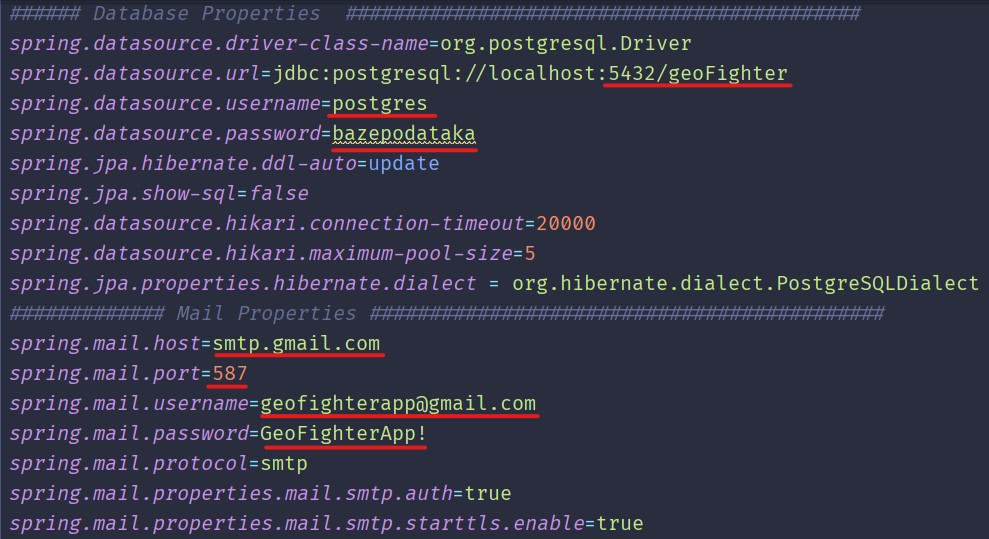
\includegraphics[scale=0.4]{slike/Properties} \\%veličina u odnosu na širinu linije
					\caption{Što promijeniti u application-local.properties}
					\label{fig:properties} %label mora biti drugaciji za svaku sliku
				\end{figure}
			
				
				\item Otvoriti konzolu i pozicionirati se unutar \textit{/izvorniKod/geoFighterSpring/} i pokrenuti naredbu \textit{"./gradlew bootRun -Dspring.profiles.active=local"} s kojom se izkompajlira i pokrene backend servis.
				
				\item Otvoriti drugu konzolu i pozicionirati se unutar \textit{/izvorniKod/angular-geofighter/} i pokrenuti naredbu \textit{"npm install"} s kojom se instaliraju sve potrebno za frontend servis. Zatim pokrenuti naredbu \textit{"ng build"}, te na kraju \textit{"npm start"} kojim se pokreće frontend servis na portu 4200.
				
				\item Ukoliko su pokrenuti backend i frontend servis i ne javlju se greške u konzoli, aplikacija je spremna za korištenje na lokalnom računalu.\\\\
				
			\end{itemize}
		
			
			\textit{Aplikacija je puštena u pogon na javno dostupnom poslužitelju \textbf{Heroku} tako da su sve tri komponente (DB, FrontEnd i BackEnd) tamo pokrenute i moguće joj je pristupiti sa linka:}\\
			\url{https://angularfrontend-release.herokuapp.com/}\\
						
			\textit{GitLab repozitorij \url{https://gitlab.com/MatejC_FER/pi} također sadrži CI/CD (Continuous integration and continuous delivery) implementiran pomoću kojeg se pri svakom commitu na \textbf{Master} branch automatski aplikacija izgradila i deployala na \textbf{Heroku} javni poslužitelj. Tako nije potrebno lokalno pokretati aplikaciju nakon izmjena, već je dovoljno na repozitorij pohraniti primjene.}
			
			
			\eject 